\documentclass[12pt]{article}
\usepackage{graphicx}
\usepackage{hyperref}
\usepackage{pdfpages}
\usepackage[margin=1in]{geometry}
\usepackage[utf8]{inputenc}
\usepackage[title]{appendix}
\graphicspath{ {./Figures/} }
\hypersetup{
    colorlinks=true,
    linkcolor=blue,
    filecolor=magenta,      
    urlcolor=cyan,
}
\urlstyle{same}
\usepackage[font={small,it}]{caption}
\usepackage{fancyvrb}
\title{Regression Analysis of Chicago Crime Volume by Ward using Public School Data}
\author{John D. Bulger, Valparaiso University\thanks{``I have neither given or received, nor have I tolerated other’s use of unauthorized aid."}}
\date{October 5, 2018}

\begin{document}
	\pagenumbering{arabic}
	\maketitle

	\section{Introduction}
	
Crime levels have been a disturbing and interesting topic for a large portion of the Chicago's history.  Infamous criminals such as Al Capone, John Dillinger, and John Wayne Gacy made names for themselves through their ``work" in the Windy City.  Within the past decade or so, Chicago’s crime rate (and homicide rate in particular) has experienced a surge.  2016 was the deadliest year in recent memory for the city.  According to Time Magazine's analysis of public data, Chicago experienced 27.7 homicides per 100,000 people, a 10-point increase over 2015.  It also outpaced the homicide rates of New York, Los Angeles, and Houston.  Additionally, all other types of crimes increased year-over-year in 2016 for Chicago as well.\cite{sanburn}

\par

Many theories attempt to explain this spike in crime (often unsuccessfully), but this analysis will explore it through the lens of public high school data.  The city of Chicago maintains an open data portal.  Official crime data by year, as well as an abundance of school data, can be easily accessed and used for analysis.  Additionally, since this data is directly reported by city agencies, it is generally viewed to be more accurate when compared to pulling data from third parties, such as news articles.

\par

The crime data and school data can be linked geographically by ward.  The city of Chicago is divided into 50 wards, which function as political districts.  While wards are not as well-recognized or segmented as Chicago’s community areas (such as Lincoln Park and Logan Square), they are adjusted after every census to ensure each one consists of approximately the same population.  While this would detract from a time-series analysis (for which community areas may be the best choice), wards should act as an effective record for this cross-sectional analysis.

\par

This analysis will focus on crime levels as a function of independent variables identified from the school data for the 2016-2017 school year.  Only crimes that occur within these time constraints will be used in creating models.  Estimates will be determined for total crime count as well as homicide count.  Since population of wards are approximately the same, a count of crimes by ward will serve as an effective, proportional target.

	\section{Prior Work}

Researchers from many disciplines have sought to shed light on the driving force that leads to crime.  While many data mining methods are capable of exploring relationships between variables driving crime, regression remains on of the most widely accepted.\cite{kaur}  This is in part due to the clearly defined effects of the independent variables on the dependent variable, which is lacking in many state-of-the-art data science algorithms (known as ``black box algorithms").

\subsection{Micro-Level}

Many instances of regression analysis on micro-level crime data have been explored and documented.  In light of the high school focus of this analysis, prior work centered on juvenile subjects is of utmost interest.  Alcohol abuse among juveniles is exhibits a statistically significant relationship with crime rates, leading researchers to suspect a possible causal effect.\cite{fergusson}  Relationships between nicotine dependence and cannabis abuse with crime have also be identified via regression analysis.\cite{ferg2}  Additionally, the association with ``deviant peers" was shown to have a significant effect on likelihood to commit a crime.  Deviant peers were measured as a scale score from the number of the subject's friends who engaged in substance abuse, received school discipline and suspensions, or who broke the law.  While the effect of peer deviation on crime likelihood appears to decrease as maturity is reached, it has a substantial effect during high school years.\cite{ferg2}

\par

A enlightening micro-level study by Azim Shariff and Mijke Rhemtulla used regression analysis to discover, in their samples, that beliefs in heaven and hell were the most influential independent variables in committing crimes, even when compared to more ``traditional" variables typically associated with crime.\cite{shariff}  The effects of the heaven and hell variables held true for a multitude of crimes, even when presented in a multivariate regression with common variables such as poverty level and amount of population incarcerated.  By evaluating the regression in this way, this study stands as a prime example of how some of the most influential variables could easily be overlooked.

\subsection{Macro-Level}

Two examples of macro-level crime regression similar in nature to this analysis focused on crime levels in Salinas, California.  The first paper, written in 2009, examines various socio-economic indicators as variables in a regression of violent crime.  These indicators included public school metrics, notably dropout rate, graduation rate, and attendance.  All of these metrics were found to have some level of relationship with crime levels.\cite{salinas_env}

\par

The second analysis built upon the previous study by taking different regression estimators (beyond OLS) and compared the results when modeled as a predictive algorithm.  In the best OLS estimate, included variables consisted of number of vacant home units, overpopulation percentage, unemployment levels, number of police officers on staff, and police department budget.\cite{salinas_crime}  While these variables do not relate to public school data, as will be examined later, this stands as an excellent example and guide to modeling crime rates via OLS on a macro-level.

	\section{Data}


\subsection{Procurement \& Preprocessing}

All of the data used in this regression analysis is freely available at the city's Open Data Portal.\cite{c1data}\cite{c2data}\cite{s1data}\cite{s2data}\cite{s3data}  The school data consisted of different metrics and information spread over three data files.  These datasets were able to be merged by school ID.  High schools were then isolated, and the variables were averaged by ward.\footnote{Not all of the 50 wards contained a high school.  So while 50 wards exist, this research only takes 48 into account.}  Imputation by median value was conducted where necessary.

\par

The crime data was contained in two datasets from 2016 and 2017.  Each record was a reported instance of a crime and contained attributes regarding location, type of crime, UCR code, and other information.  The two years of data were combined; then, crimes that occurred outside of the 2016-2017 school year were dropped.  The total number of crimes, as well as the total number of homicides, were summed by ward.  A visual representation of this crime distribution by ward can be seen in Appendix A.  The school data was then joined to the crime data by ward to create the final dataset used in this regression analysis.\footnote{This data preprocessing was conducted using R and Python.  Scripts and data can be found in the GitHub repository for this project at \href{https://github.com/jdbul33/reimagined-parakeet}{https://github.com/jdbul33/reimagined-parakeet}.}


\subsection{Variables}

\paragraph{Dependent Variables}
Relevant variables were chosen from this final dataset, upon which the regression will be built.  The two dependent variables were identified as total crime instances and total homicide count by ward for the 2016-2017 school year.  The basic statistical description of these variables can be seen in Table 1.

\begin{center}
	\begin{table}[h]
	\begin{tabular}{ c | c | c | c | c | c }
		
		 & \textbf{Mean} & \textbf{Median} & \textbf{Std. Dev.} & \textbf{Minimum} & \textbf{Maximum} \\ 
		 \hline
		 \textbf{Total Crime} & 4,194 & 3,280 & 2327 & 1,824 & 12,057 \\
		 \textbf{Homicides} & 12 & 7.5 & 11.7 & 0 & 45 \\
    
	\end{tabular}
\caption{Descriptive statistics of the dependent variables for Chicago by ward}
\end{table}
\end{center}  

\paragraph{Independent Variables}
Independent variables were then identified from the dataset based on theory, prior work on this subject, and availability.  OLS necessitates that all variables used with the estimator must be stated numerically; therefore, all chosen variables are either numeric or able to be translated as such.\footnote{Dress Code is a dummy, binary variable.  Schools with a dress code are valued at 1, while those without a dress code are denoted by 0.  Therefore, each ward will have a dress code value of 0-1, depending on the mix of high schools in that ward.}\footnote{Survey variables result from surveys given to teachers and students to rank their school in five criteria:  supportive environment, involved families, school safety, collaborative teaching, and ambitious instruction.  Scoring is from 0-5 with 5 being the best.}  This precluded many free-format data fields consisting of comments or non-ordinal evaluation.  The chosen variables and their descriptive statistics can be seen in Table 2.  This list consists of the initial variables that were evaluated for regression analysis, not the final model's variables.
\par
These variables were then evaluated for correlation, as correlated independent variables violate one of the basic assumptions of OLS.  This was completed visually (since the number of variables chosen was relatively small) utilizing R, a statistical software.  The resulting correlations can be seen in the correlation matrix in Figure 1.  This information was referenced as final variables were selected.

\begin{center}
	\begin{table}[h]
		\begin{tabular}{ c | c | c | c | c | c }
			
			& \textbf{Mean} & \textbf{Median} & \textbf{Std. Dev.} & \textbf{Minimum} & \textbf{Maximum} \\ 
			\hline
			\textbf{Graduation Rate} & 72.9\% & 74.6\% & 13.7\% & 27.8\% & 93.5\% \\
			\textbf{College Enrollment} & 49.3\% & 50.2\% & 18.0\% & 10.8\% & 85.7\% \\
			\textbf{Dress Code} & 0.6 & 0.6 & 0.4 & 0 & 1\\
			\textbf{Average ACT Score} & 17.0 & 16.8 & 2.2 & 13.1 & 22.3\\
			\textbf{Survey-Supportive} & 3.3 & 3.4 & 0.7 & 1 & 5\\
			\textbf{Survey-Families} & 3.2 & 3.2 & 1 & 0 & 5\\
			\textbf{Survey-Leadership} & 3.1 & 3.2 & 0.9 & 0 & 5\\
			\textbf{Survey-Safety} & 2.1 & 2 & 0.6 & 0.5 & 3.7\\
			\textbf{Survey-Teachers} & 3.5 & 3.5 & 0.9 & 0 & 5\\
			\textbf{Survey-Instruction} & 3.7 & 4 & 0.8 & 1.5 & 5\\
			\textbf{Student Attendance} & 85.5\% & 87.8\% & 7.6\% & 53.8\% & 95.4\% \\
			\textbf{Teacher Attendance} & 92.5\% & 92.6\% & 0.6\% & 91.1\% & 93.6\% \\
			\textbf{Suspensions/100 stud.} & 22.5 & 16.6 & 19 & 0.6 & 103\\
			\textbf{Dropout Rate} & 10.3\% & 7.2\% & 8.7\% & 0.9\% & 33.4\% \\
			\textbf{Low Income Students} & 85.5\% & 90.2\% & 10.8\% & 54.3\% & 95.7\% 
			
		\end{tabular}
		\caption{Descriptive statistics of candidate independent variables for Chicago high schools by ward}
	\end{table}
\end{center}

	\begin{figure}[h]
		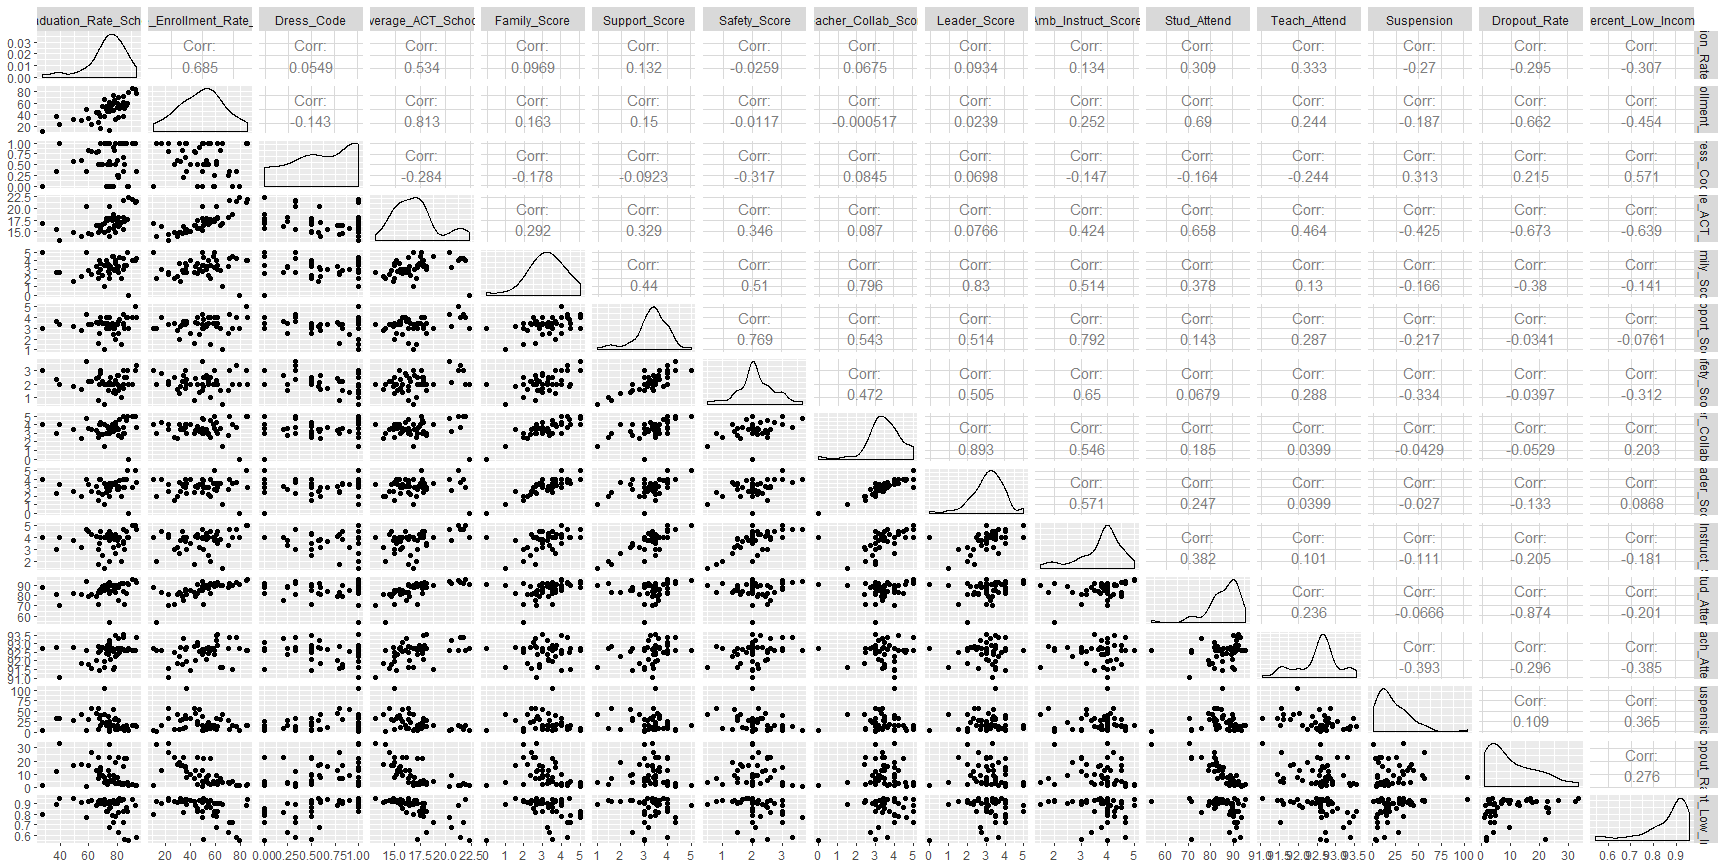
\includegraphics[scale=.33]{pairplot.png}
		\caption{Visualization of correlations and distributions of candidate independent variables}
	\end{figure}

\subsection{Variable Selection, Model Specification, \& Model Estimation}

The model chosen to explain crime as a function of public school data was a linear regression using Ordinary Least Squares as the estimator.  Exploratory analysis of the target variables and the literature review suggests that a linear relationship is the most fitting for this analysis.  Furthermore, each ward has essentially the same population, so total crime count by ward represents a consistent rate, eliminating the need to standardize it.

\par

The variables shown in Table 2 represent all of the possible attributes from the data that could theoretically serve as a predictor and that could be coded in a numeric format, as explained earlier.  In order to narrow these variables into an initial model, stepwise regression was utilized.  This was conducted using R, with a separate analysis conducted for each of the dependent variables:  total crime and total homicides.  Once completed, these selected variables were analyzed as a regression in SAS, tested for multicollinearity and heteroscedasticity, and  subsequently worked into the best possible model given the data.

\paragraph{Total Crime}

The stepwise regression for this analysis used Total Crime as the dependent variable and all of the initial variables in Table 2 as a starting point.  After running this analysis, the independent variables detected as most important were identified as graduation rate, college enrollment rate, dress code, effective leadership survey score, average ACT score, involved family survey score and dropout rate.  Upon examination using correlations in Figure 1, the two survey score variables were found to have a correlation coefficient of 0.83.  This is above a commonly used threshold of 0.8, and thus supportive family survey score was dropped from the estimated model.  This was chosen from the two variables after comparing regression results after omitting each of the two variables, using adjusted R-squared as the measure.  The aforementioned variables were then run using \textit{PROC REG}, the regression command in SAS.  Upon evaluation, average ACT score and the leadership survey variables stood out with high p-values of 0.90 and 0.19, respectively.  When viewed through a theoretical lens, these two variables were not identified as necessary.  As a result, they were then dropped from the estimate.  Other variables, such as suspensions per 100 students, were worked in and out of the regression in an attempt to eliminate any omitted variable bias.  None of these added any statistical basis to the regression.  Additionally, given the exploratory nature of this analysis, no variables are absolutely necessary on a theoretical basis.  The regression specification, prior to estimation, is as follows:

\begin{center}
\begin{math}
\hat{TotalCrime} = \hat{\beta_{0}}+\hat{\beta_{1}}GraduationRate+\hat{\beta_{2}}CollegeEnrollment+\hat{\beta_{3}}DressCode+\hat{\beta_{4}}DropoutRate+\epsilon_{i}
\end{math}
\end{center}

The final variable metrics are shown in Table 3, and the resulting estimate equation can be written as: \\

\begin{center}
\begin{math}
TotalCrime = 2185 - 62.22*GraduationRate + 73.35*CollegeEnrollmentRate + 2451.65*DressCode + 138.44*DropoutRate
\end{math}
\end{center}


\begin{center}
	\begin{table}[h]
		\begin{tabular}{ c | c | c | c | c }
			
			& \textbf{Grad. Rate} & \textbf{College Enroll} & \textbf{Dress Code} & \textbf{Dropout Rate} \\
			\hline
			\textbf{Coefficient Estimate} & -62.22 & 73.35 & 2451.65 & 138.44 \\
			\textbf{Standard Error} & 31.16 & 29.95 & 844.39 & 47.29 \\
			\textbf{T-Statistic} & -2.00 & 2.45 & 2.90 & 2.93\\
			\textbf{P-Value} & 0.0522 & 0.0185 & 0.0058 & 0.0054		
		\end{tabular}
		\caption{Coefficients, standard error, and p-values for linear regression of total crime}
	\end{table}
\end{center}

\paragraph{Total Homicides}

The same variables shown in Table 3 were fit to total homicides as the target variable.  With less occurrences, and in some wards no occurrences, this model fitting was conducted as with lower expectations for regression quality.  In order to build a more accurate model, more robust homicide data is necessary.  The variable statistics can be seen in Table 4, and the resulting regression estimate was determined to be:
\\
\begin{center}
\begin{math}
TotalHomicides = 16.3 - 0.236*GraduationRate + 0.045*CollegeEnrollmentRate + 12.125*DressCode + 0.305*DropoutRate $$
\end{math}
\end{center}

\begin{center}
	\begin{table}[h]
		\begin{tabular}{ c | c | c | c | c }
			
			& \textbf{Grad. Rate} & \textbf{College Enroll} & \textbf{Dress Code} & \textbf{Dropout Rate} \\
			\hline
			\textbf{Coefficient Estimate} & -0.236 & 0.045 & 12.125 & 0.305 \\
			\textbf{Standard Error} & 0.161 & 0.155 & 4.375 & 0.245 \\
			\textbf{T-Statistic} & -1.46 & 0.29 & 2.77 & 1.25\\
			\textbf{P-Value} & 0.1505 & 0.7737 & 0.0082 & 0.2193		
		\end{tabular}
		\caption{Coefficients, standard error, and p-values for linear regression of total homicides}
	\end{table}
\end{center}



	\section{Analysis of Regression Estimate Quality}


	\subsection{Total Crime Regression}
	
	\paragraph{Theory}
	When the equation estimate is viewed through the lens of theoretical relationship, it perhaps seems somewhat counterintuitive at first.  However, most of the variables' relationship to the number of total crimes can be rationalized.  It is important to note, however, that the presence of a relationship does not necessarily indicate causation.  Schools with a lower graduation rates support the theory that students with less options for a future (like not possessing a high school diploma) may be more inclined to get involved with criminal activity.  This is reflected in that variable's negative coefficient.  Dress code should theoretically reduce crime by making gang affiliations less apparent, yet it has a positive relationship with crime count.  It could be the case that institution of a dress code is reactionary to crime; that is, schools in higher crime areas require a dress code in order to help with the issue.  Dropout rate has a positive relationship with crime, which furthers the argument that students with less options are perhaps more inclined to engage in crime.
	
	\par
	
	College enrollment is the one variable that is perhaps not explainable on a theoretical level.  Common sense indicates that college-bound students are perhaps less engaged in criminal activity than non-college-bound students.  Similarly, higher-crime areas would be expected to have less families with a college graduate than lower-crime areas.  However, the variable is shown to be statistically significant, and further research may be necessary to explore this relationship.
	
	\paragraph{Fit}

	The linear model for total crime exhibits a reasonable level of fit.  It has a $ R^{2} $ value of 0.3154 and a $ \bar{R}^{2} $ of 0.2518.  Both metrics measure overall fit on a scale from 0-1, with $ \bar{R}^{2} $ ``penalizing" for the addition of more variables.  Since this is a multivariate regression, both metrics must be taken into account.  The values for these suggest that this is a model that is indeed indicative of a relationship..
	
	\par
	
	Furthermore, all variables in this regression estimate have p-values that are low enough to be considered statistically significant.  A p-value serves as a measure to reject the null hypothesis, that the expected variable coefficient is 0, based on the variable's t-value.  For this analysis, a standard p-value of less than 0.05 is considered to be significant.  Since all of the variables exhibit this, the null hypothesis, which states that the coefficient is expected to be zero, is rejected.
	
	\par
	
	A regression's F-value is a measure of the model's overall significance when compared to the null hypothesis, which states that the expected coefficients for all of the variables is zero.  While the F-value can range from 0 to an arbitrarily large number, the best measure of its significance is its corresponding p-value.  In this regression model, the p-value was found to be 0.0023.  This is well below the established threshold of 0.05 for statistical significance, and the null hypothesis is rejected.

	\paragraph{Potential Issues}All variables included in the total crime regression pass the White test for heteroscedasticity and have suitably low Variance Inflation Factors, as can be seen in Table 4.  The White adjustment for heteroscedasticity shows that all of the included variables maintain an acceptably low p-value and standard error.  A Variance Inflation Factor of less than 5 is typically accepted as not indicative of severe multicollinearity, and all of the included variables fall below this limit.

	\begin{center}
		\begin{table}[h]
			\begin{tabular}{ c | c | c | c | c }
				
				& \textbf{Coefficient Est.} & \textbf{Adj. Std. Error} & \textbf{Adj. P-Value} & \textbf{VIF} \\
				\hline
				\textbf{Graduation Rate} & -62.22 & 27.57 & 0.029 & 2.12  \\
				\textbf{College Enrollment} & 73.35 & 28.55 & 0.014 & 3.38 \\
				\textbf{Dress Code} & 2451.65 & 718 & 0.001 & 1.08 \\
				\textbf{Dropout Rate} & 138.43 & 51.07 & 0.010 & 1.96
				
			\end{tabular}
			\caption{Heteroscedasticity and multicollinearity test results for linear regression model of total crime}
		\end{table}
	\end{center}
	

	\subsection{Total Homicide Regression}

	\paragraph{Theory \& Fit}  In the linear regression for total homicides, the variables all exhibited coefficients with the same indication of relationship.  Therefore, the theory explained and rationalized above extrapolates to this model as well.  The estimate's fit, however, is not as strong as the primary model.  The regression yielded a $ R^{2} $ of 0.2791 and a $ \bar{R}^{2} $ of 0.212.  These metrics are not as high as in the initial regression, suggesting that the regression does not exhibit as good of a fit.  The model has a F-value of 4.16 with a corresponding p-value of 0.0062, which shows the null hypothesis (that all expected variable coefficients should be zero) is rejected.
	
	\paragraph{Potential Issues}
	
	As with the prior model, the regression estimate for total homicides was subjected to standard tests for multicollinearity and heteroscedasticity.  Since the same variables were examined, the Variance Inflation Factors, indicators of multicollinearity, remain the same at acceptably low levels.  White's test was used to produce standard errors for the coefficients and the resulting  p-values after adjusting for any heteroscedasticity.  Some change can be seen, but it does not change the p-values by a large margin from where they were originally.
	\begin{center}
	\begin{table}[h]
		\begin{tabular}{ c | c | c | c | c }
			
			& \textbf{Coefficient Est.} & \textbf{Adj. Std. Error} & \textbf{Adj. P-Value} & \textbf{VIF} \\
			\hline
			\textbf{Graduation Rate} & -0.236 & 0.146 & 0.1122 & 2.12  \\
			\textbf{College Enrollment} & 0.045 & 0.132 & 0.7346 & 3.38 \\
			\textbf{Dress Code} & 12.125 & 3.153 & 0.0004 & 1.08 \\
			\textbf{Dropout Rate} & 0.305 & 0.201 & 0.1366 & 1.96
			
		\end{tabular}
		\caption{Heteroscedasticity and multicollinearity test results for linear regression model of total homicides}
	\end{table}
\end{center}

	\section{Discussion}

The results from this regression analysis show that public school metrics can indeed be linked to crime and homicide rates in the city of Chicago.  Beyond theoretical significance, it is evident that the chosen variables exhibit statistical significance as well.  When these two aspects of support are viewed in tandem, it paints a strong case for the relationship of school metrics to crime levels.

\par
Since this regression in linear in nature, the coefficients in the estimates can be explained simply.  For each 1\% increase in college enrollment, graduation rate, and dropout rate, crime levels are estimated to increase or decrease by the amount of the respective coefficient, all else held equal.  Dress code, on the other hand, measures the average dress code coherence within a ward.  For a change in this variable, crime will increase or decrease by the amount of the coefficient, all else held equal.  The amount of change in the dress code variable will differ based on how many schools are in the ward (since it is essentially an average).


	\section{Conclusions}

In conclusion, this analysis can be seen as a success.  A statistically significant regression estimate, using theoretically sound variables, was able to be created from the Chicago Public School data.  This estimate serves as a sensible initial explanation of the relationship of the data to crime and homicide levels.

\par

Through the results obtained, Chicago may be able to gain deeper insights into its crime problem.  However, it should be reinforced that a regression does not necessarily indicate causation; it serves only to quantify a relationship.  Dress code, in this estimate, exhibits a positive relationship with crime; if more schools in a ward require a dress code, crime levels are predicted to be higher (all else held constant).  However, it is not theoretically sound to state that removing all dress codes would lower crime; rather, dress code institution may serve as an existing measure to mitigate crime levels in at-risk areas.  Dropout rate and graduation rate both have expected relationships with crime levels, so schools and administrators should continue to emphasize the importance of scholarship and success to their students.

\par

From this regression analysis alone, no solid policy recommendations can be put forth.  The nature of this analysis was exploratory, and the data set size was relatively limited.  Additionally, the nature of the publicly available school data focuses on metrics.  While these metrics can and do show a relationship to crime, they could either exist as either a cause of or an effect of crime levels.  The theory can function either way (i.e. low graduation rates lead to more crime, or more crime leads to lower graduation rates).  



\subsection{Opportunities for Further Work}

In order to gain a deeper knowledge that could be of actionable use to city officials, a different (and perhaps deeper) analysis is necessary.  This could be accomplished in several ways.  First, while publicly available metrics show a relationship, perhaps nonpublic school data (such as budget, after-school program participation, etc.) could show variables that officials have direct control over.  With more differing variables to choose from, a stronger regression could be estimated.

\par

Secondly, this analysis only focused on the public school data.  While socioeconomic indicators are frequently studied in regards to crime, perhaps a logical next step would be to combine variables such as income, poverty level, and racial diversity with the public school data.  Since these ``traditional" variables are frequently tied to crime, and school data now can be as well, a more meaningful result may lie in some combination of the two.

\par

Lastly, a different estimation method on a larger data set may yield different, less obvious insights.  For example, crime could be potentially broken down by high school area, so that each high school represented a data point (a significant increase in observations from 48 wards).  On this more robust data, different estimators and model-building algorithms, such as random forests, could be utilized.  Such methodology may reveal relationships not theorized and thus excluded from a linear regression.





\newpage

\begin{appendices}
	
\section{Visualization of Interactive Data Map}


\begin{figure}[h]
	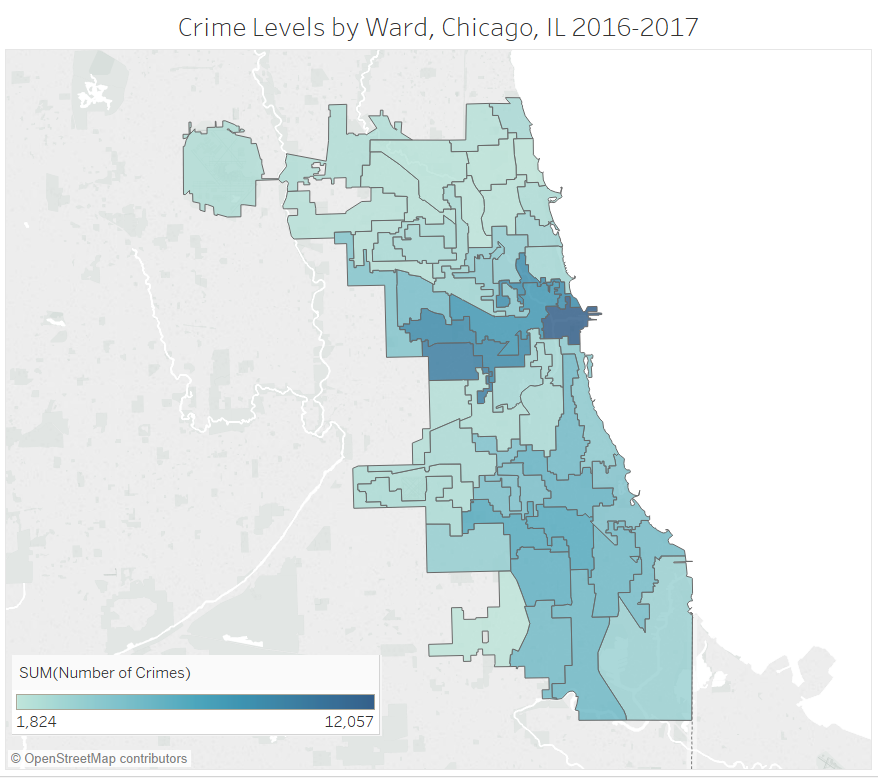
\includegraphics[scale=.9]{map_plot.png}
\end{figure}

\newpage
\section{Linear Regression for Total Crime:  SAS Output}
	
\includepdf[pages=-]{Figures/linear_total_crime_regression.pdf}

\section{Linear Regression for Total Homicides:  SAS Output}

\includepdf[pages=-]{Figures/linear_total_homicides_regression.pdf}
	

\end{appendices}






	\newpage
	\begin{thebibliography}{12}
	
\bibitem{sanburn}
Sanburn, J. and Johnson, D. (2017, January). See Chicago's Deadly Year in 3 Charts. \textit{Time}. Retrieved from \href{http://time.com/4635049/chicago-murder-rate-homicides}{http://time.com/4635049/chicago-murder-rate-homicides}.

\bibitem{kaur}
Kaur, S. and Singh, W. (2017). Systematic review of crime data mining. \textit{International Journal of Advanced Research in Computer Science, 8}(5).

\bibitem{fergusson}
Fergusson, D.M. and Horwood, L.J. (2000). Alcohol abuse and crime: a fixed-effects regression analysis. \textit{Addiction, 95}(10), 1525-1536.

\bibitem{ferg2}
Fergusson, D.M., Swain-Campbell, N.R., and Horwood, L.J. (2002). Deviant peer affiliations, crime, and substance use: a fixed effects regression analysis. \textit{Journal of Abnormal Child Psychology, 30}(4), 419-430.

\bibitem{shariff}
Shariff, A.F. and Rhemtulla M. (2012). Divergent effects of beliefs in heaven and hell on national crime rates. \textit{PLoS ONE, 7}(6). \href{https://doi.org/10.1371/journal.pone.0039048}{https://doi.org/10.1371/journal.pone.0039048}.

\bibitem{salinas_env}
Clarke, J.A. and Onufer, T.L. (2009). Understanding environmental factors that affect violence in Salinas, California. \textit{Calhoun: The NPS Institutional Archive}. Retrieved from \href{http://hdl.handle.net/10945/4466}{http://hdl.handle.net/10945/4466}.

\bibitem{salinas_crime}
Shingleton, J.S. (2012). Crime trend prediction using regression models for Salinas, California. \textit{Calhoun: The NPS Institutional Archive}. Retrieved from \href{http://hdl.handle.net/10945/7416}{http://hdl.handle.net/10945/7416}.

\bibitem{c1data}
City of Chicago. (2018). \textit{Crimes - 2016}[Data file]. Retrieved from \href{https://data.cityofchicago.org}{https://data.cityofchicago.org}.

\bibitem{c2data}
City of Chicago. (2018). \textit{Crimes - 2017}[Data file]. Retrieved from \href{https://data.cityofchicago.org}{https://data.cityofchicago.org}.

\bibitem{s1data}
City of Chicago. (2018). \textit{Chicago-Public-Schools-School-Locations-SY1617}[Data file]. Retrieved from \href{https://data.cityofchicago.org}{https://data.cityofchicago.org}.

\bibitem{s2data}
City of Chicago. (2017). \textit{Chicago Public Schools - School Progress Reports SY1617}[Data file]. Retrieved from \href{https://data.cityofchicago.org}{https://data.cityofchicago.org}.

\bibitem{s3data}
City of Chicago. (2017). \textit{Chicago Public Schools - School Profile Information SY1617}[Data file]. Retrieved from \href{https://data.cityofchicago.org}{https://data.cityofchicago.org}.

	\end{thebibliography}

\end{document}